\documentclass[../main.tex]{subfiles}
\graphicspath{{\subfix{../images/}}}
\begin{document}

\subsection{Increasing Network Complexity}
\subsubsection{Increasing Layer}

The model of AlexNet was adopted and changed to create the base of the model. The network was increased to a network with 4 layers while using similar techniques such as decreasing convolutional kernel sizes and strides. 

\subsubsection{Dropout Layer}

The paper for the AlexNet model discussed the use of the dropout layer technique which was used to prevent overfitting. 

\begin{figure}[h!]
  \centering
  \begin{subfigure}[b]{0.35\linewidth}
    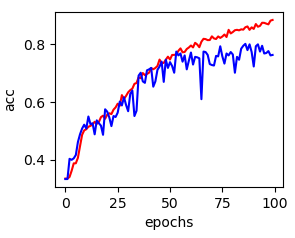
\includegraphics[width=\linewidth]{without-dropout.png}
    \caption{Without Dropout}
  \end{subfigure}
  \begin{subfigure}[b]{0.35\linewidth}
    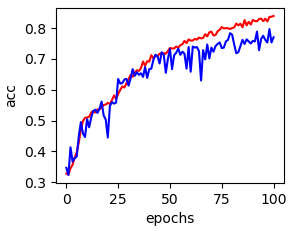
\includegraphics[width=\linewidth]{withdo.png}
    \caption{With Dropout}
  \end{subfigure}
  \caption{Dropout Performance}
  \label{fig:dropout-performance}
\end{figure}

We see that for both graphs, the model starts to become overfit as the rate the training set accuracy is improving become greater than the validation set. However, we see that with dropout, this 'branching out effect' is minimised whereas the first graph converges to an accuracy of around 75\%. It is predicted that with more epochs, the model with dropout will achieve a greater accuracy than without dropout.

\subsubsection{Pooling Layer}

Similar to what was used in AlexNet, the use of the overlapped pooling technique was used in the model. A pooling layer using a size 3 kernel and the stride of 2 was tested.

\begin{figure}[h!]
  \centering
  \begin{subfigure}[b]{0.35\linewidth}
    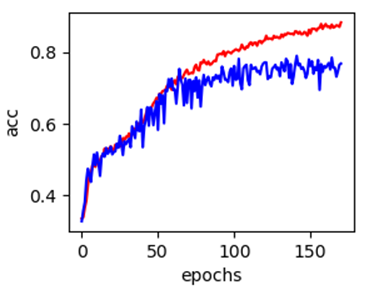
\includegraphics[width=\linewidth]{withdo-without-pool.png}
    \caption{With Normal Pooling}
  \end{subfigure}
  \begin{subfigure}[b]{0.35\linewidth}
    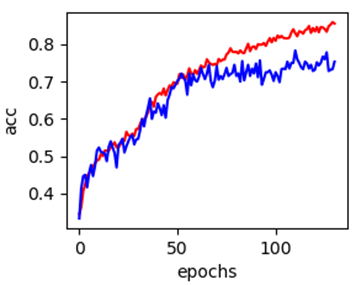
\includegraphics[width=\linewidth]{withdo-overlap-pooling.png}
    \caption{With Overlapping Pooling}
  \end{subfigure}
  \caption{Overlapping Pooling Performance}
  \label{fig:pooling-performance}
\end{figure}

We see on Figure \ref{fig:pooling-performance}, with the regular pooling, the model achieved an accuracy of 70\% whereas with overlapping pooling, the accuracy was close to 75\% which is a 5\% improvement. Hence this technique is effective in improving the accuracy of the model.

\end{document}